\subsection{\gls{uefi}/\gls{pi} Firmware Images}
\gls{uefi} and \gls{pi} specifications define the standardized format for EFI firmware storage devices (FLASH or other non-volatile storage) which are abstracted into "Firmware Volumes". Build systems must be capable of processing files to create the file formats described by the \gls{uefi} and PI specifications. The tools provided as part of the \gls{edk2} BaseTools package process files compiled by third party tools, as well as text and Unicode files in order to create UEFI or PI compliant binary image files. In some instances, where UEFI or PI specifications do not have an applicable input file format, such as the Visual Forms Representation (VFR) files used to create PI compliant IFR content, tools and documentation have been provided that allows the user to write text files that are processed into formats specified by UEFI or PI specifications.

\begin{figure}[h]
	\centering
	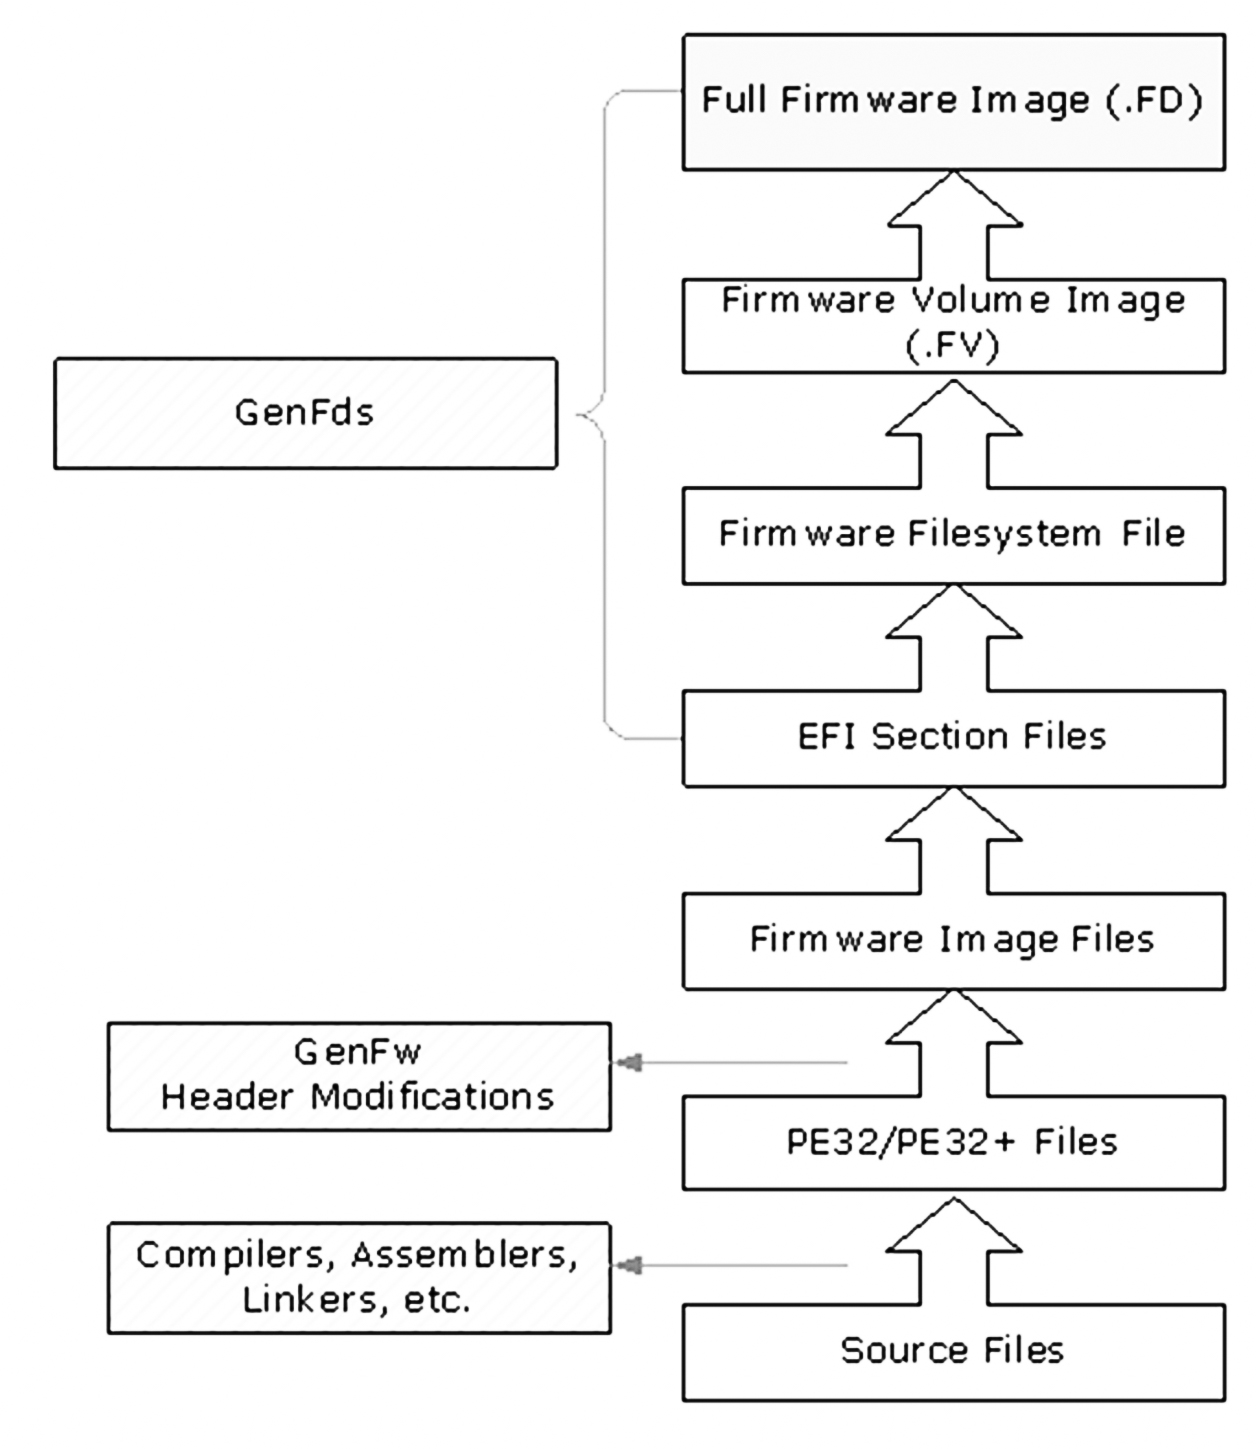
\includegraphics[width=0.7\linewidth]{design/uefi-pi-firmware-image-creation}
	\caption{UEFI/PI Firmware Image Creation}\label{fig:design-uefi-pi-firmware-image-creation}
\end{figure}

A Firmware Volume (FV) is a file level interface to firmware storage. Multiple FVs may be present in a single FLASH device, or a single FV may span multiple FLASH devices. An FV may be produced to support some other type of storage entirely, such as a disk partition or network device. For more information consult the Platform Initialization Specification, Volume 3.
In all cases, an FV is formatted with a binary file system. The file system used is typically the Firmware File System (FFS), but other file systems may be possible in some cases. Hence, all modules are stored as "files" in the FV. Some modules may be "execute in place" (linked at a fixed address and executed from the ROM), while others are relocated when they are loaded into memory and some modules may be able to run from ROM if memory is not present (at the time of the module load) or run from memory if it is available.
Files themselves have an internally defined binary format. This format allows for implementation of security, compression, signing, etc. Within this format, there are one or more "leaf" images. A leaf image could be, for example, a PE32 image for a DXE driver.

Therefore, there are several layers of organization to a full UEFI/PI firmware image. These layers are illustrated below in Figure \ref{fig:design-uefi-pi-firmware-image-creation}. Each transition between layers implies a processing step that transforms or combines previously processed files into the next higher level. Also shown in Figure \ref{fig:design-uefi-pi-firmware-image-creation} are the reference implementation tools that process the files to move them between the different layers.

\begin{figure}[h]
	\centering
	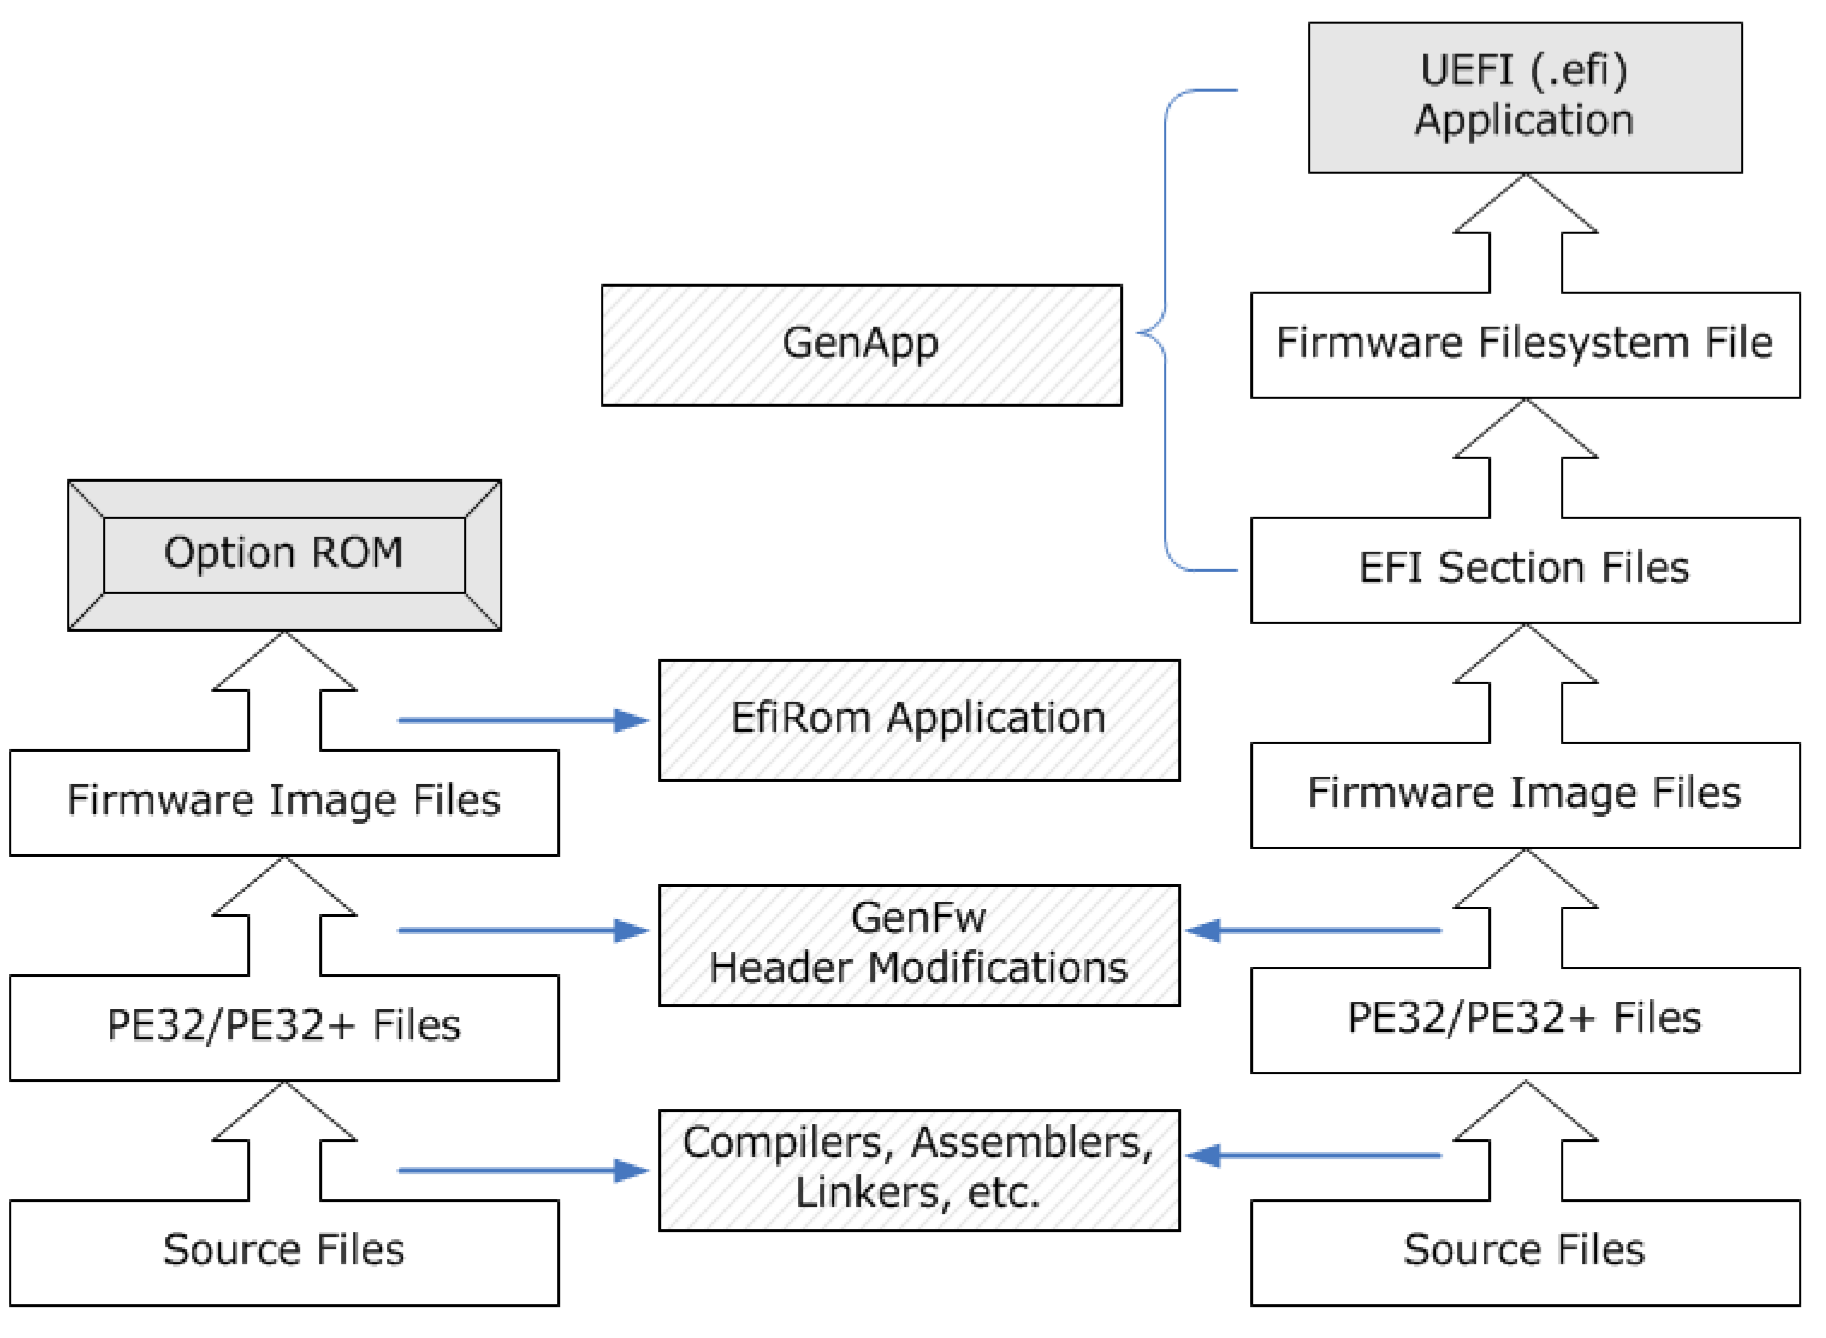
\includegraphics[width=0.7\linewidth]{design/efi-application-creation}
	\caption{UEFI/PI Firmware Image Creation}\label{fig:design-efi-application-creation}
\end{figure}


In addition to creating images that initialize a complete platform, the build process also supports creation of stand-alone UEFI applications (including OS Loaders) and Option ROM images containing driver code. Figure \ref{fig:design-efi-application-creation}, below, shows the reference implementation tools and creation processes for both of these image types

The final feature that is supported by the EDK II build process is the creation of Binary Modules that can be packaged and distributed for use by other organizations. Binary modules do not require distribution of the source code. This will permit vendors to distribute UEFI images without having to release proprietary source code.

This packaging process permits creation of an archive file containing one or more binary files that are either Firmware Image files or higher (EFI Section files, Firmware File system files, etc.). The build process will permit inserting these binary files into the appropriate level in the build stages.